\section{Development and Configuration Selection}
The development study used Replica office\_0 and office\_1 and SceneNN 014 and 015, all previously examined in the project. Its original primary configuration required three refutation frames. The one-refutation arm was selected before processing the four new SceneNN sequences and is the \ours{} configuration in the main paper. Development scores are not independent test evidence and are not pooled with the main table.



\paragraph{Selection rule and chronology.} The original pilot fixed three refutations as primary and evaluated a one-refutation control. After observing development results, we selected that existing control empirically: its dataset-mean gains were $+2.018$ and $+1.034$, versus $+2.002$ and $+0.656$ for three refutations, and it gained one match without losing any in each dataset. Only the minimum count changed from three to one; the depth gate, two-pixel boundary, and $R\geq2S$ rule stayed fixed. This was a development-informed choice, not a preregistered automatic selection algorithm. The separate new-scene protocol then fixed this arm before RGB processing and scoring. Selection did not make the original pilot pass its two-point-per-dataset requirement, nor did it remove the subsequent SOR deficit.

On the two Replica development scenes, the scene-macro mean increases from $38.971$ to $40.989$ ($+2.018$ points), compared with $39.501$ for SOR. On the two SceneNN development scenes, it increases from $15.138$ to $16.171$ ($+1.034$), compared with $15.561$ for SOR. The pilot one-refutation arm gains one match and loses none in each dataset. This does not imply a recall gain on the new test sequences, where the matched set is unchanged.

The original three-frame development configuration failed its dataset-gain and persistence checks. The new-sequence primary configuration also did not pass the predeclared beats-SOR check. These outcomes remain part of the evidence record. No additional configuration was selected after the new-sequence scores were observed.

\section{Relationship to Point-Ratio Filtering}
For nonnegative integer vote counts with $S+R>0$, the primary rule has the equivalent form
\begin{equation}
R\geq1\ \land\ R\geq2S\quad\Longleftrightarrow\quad
\frac{S}{S+R}\leq\frac13.
\end{equation}
The zero-evidence case $S=R=0$ is retained. Equality was checked against the actual rejection function for all 20,301 pairs with $S+R\leq200$. This is a code/mathematical consistency check, not an additional mapping experiment.

The pinned MaskClustering point filter computes a detection ratio whose numerator counts cluster support and whose denominator counts point presence in node-visible frames. Its configuration here retains ratios strictly above $0.5$. That system also includes splitting and object-level retention. Our denominator counts only decisive support/refutation observations after depth and boundary gating; observation membership and identities remain fixed. Thus the numerical thresholds should not be compared without accounting for the different evidence domains and representations.

The adapted system comparison does not isolate the two point filters under identical masks and object ownership. It supports a comparison of the exported maps under the common evaluator, not a claim that our ratio alone outperforms the competing filter. The depth ablation probes one component of the proposed evidence domain.

\section{Reproduction and Display Protocol}
All primary tables are generated from the frozen per-scene metrics; per-object and threshold-case tables are generated from their stored diagnostic records. The document package contains source hashes and a figure manifest. Document regeneration loads no model checkpoint, launches no mapping job, and changes no saved prediction.

The main paper evaluates exclusive label transfer within $5\,\mathrm{cm}$ on the fixed observed-valid domain. For dense qualitative context only, foreground instance IDs can be displayed on nearby scene points within $3\,\mathrm{cm}$. This display operation does not change the prediction files or evaluation radius. Scene-view figures use calibrated camera projections; same-object comparisons use a shared orthographic orientation and common axis bounds. Selected illustrative objects and frames are post-hoc examples.

The controlled RGB-D branch uses given poses and SAM2.1/SigLIP observations. Archived robot maps have distinct branch identities and map coordinate revisions. Garage object evidence is kept in its original \texttt{omni\_odom} coordinates; outdoor object evidence uses its own stored corrected-map revision. Geometry from those revisions is not mixed. The six-route atlas separately uses the reviewed offline-backend maps.

The accompanying source archive is sufficient to compile the paper and supplement from included figure assets and tables. Repeating the original experiments additionally requires the datasets, models, cached observations, and frozen source environment; the document archive alone is not an experimental container.

\clearpage
\onecolumn
\section*{Development and Instance-Level Results}
\begin{table}[h!]
\centering
\caption{Development scores (PQ $\times100$). The pilot no-depth variant requires three refutations; it differs from the one-refutation no-depth ablation in the main paper.}
\label{tab:development}
\begin{tabular}{lrrrrr}
\toprule
Scene & Baseline & SOR & Three-frame & No depth (3) & Ours (1) \\
\midrule
office\_0 & 30.923 & 31.249 & 34.017 & 33.589 & 34.078 \\
office\_1 & 47.019 & 47.752 & 47.928 & 45.289 & 47.900 \\
SN 014 & 15.868 & 16.452 & 17.133 & 17.068 & 17.824 \\
SN 015 & 14.408 & 14.669 & 14.454 & 14.422 & 14.519 \\
\bottomrule
\end{tabular}

\end{table}

\begin{figure}[h!]
\centering
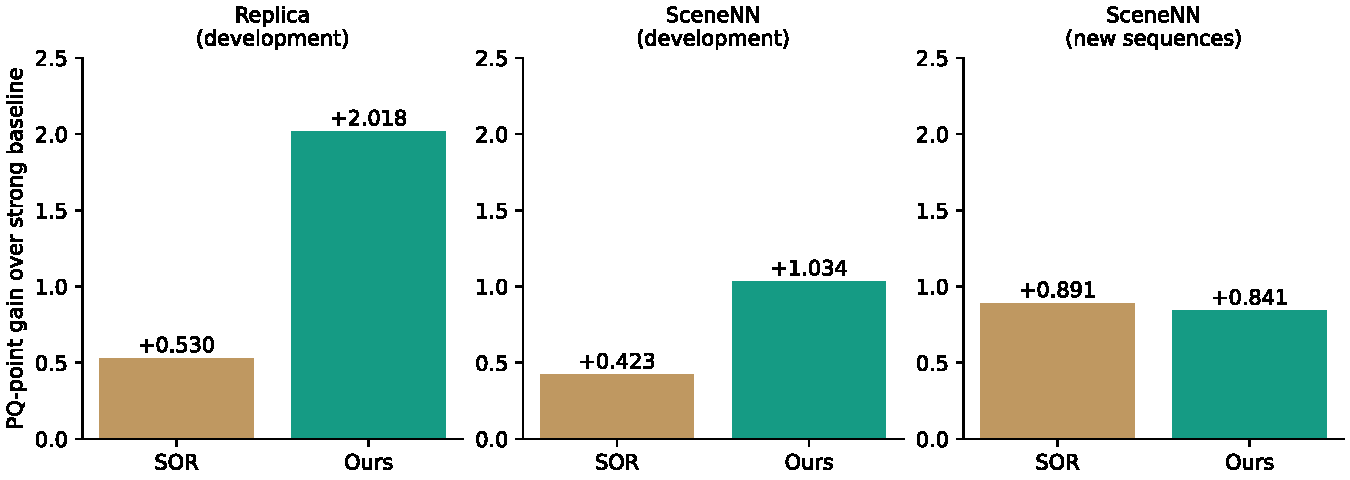
\includegraphics[width=.92\textwidth]{development_vs_unseen.pdf}
\caption{Gains over the corresponding strong baseline, separated by dataset and development exposure. Only the final group contains the four new SceneNN sequences used in the main result table.}
\end{figure}

\begin{figure}[h!]
\centering
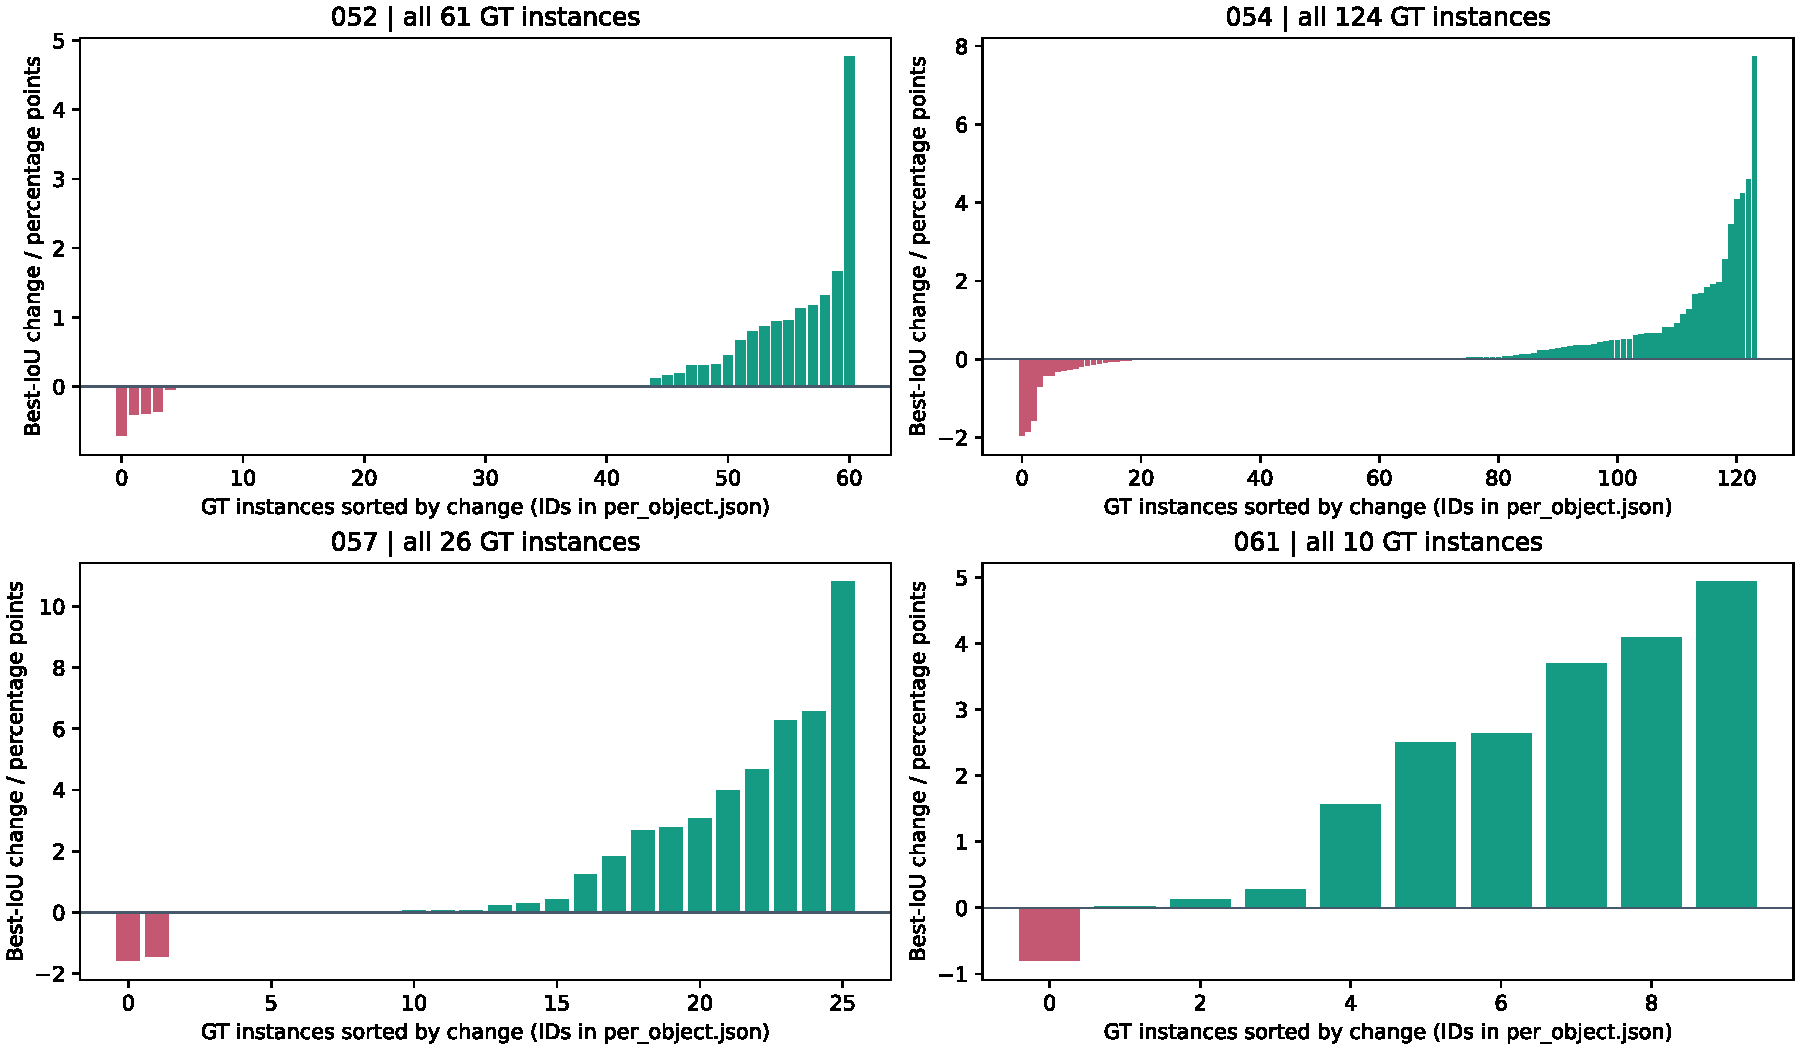
\includegraphics[width=.92\textwidth]{all_object_changes.pdf}
\caption{Best-object IoU changes for all 221 ground-truth instances. Instances are sorted by change within each scene; unchanged and regressed objects are retained. This display does not treat within-scene objects as independent statistical trials.}
\end{figure}

\clearpage
\section*{Evidence and Assignment Diagnostics}
The plots below separate the source of the sequence-057 deficit from the effect of reference-label assignment. One SOR-only match outweighs gains on the remaining objects. Fixing the original source owner changes the ranking, so the primary and locked-assignment results should be interpreted together; the primary evaluator remains unchanged.

\begin{figure}[h!]
\centering
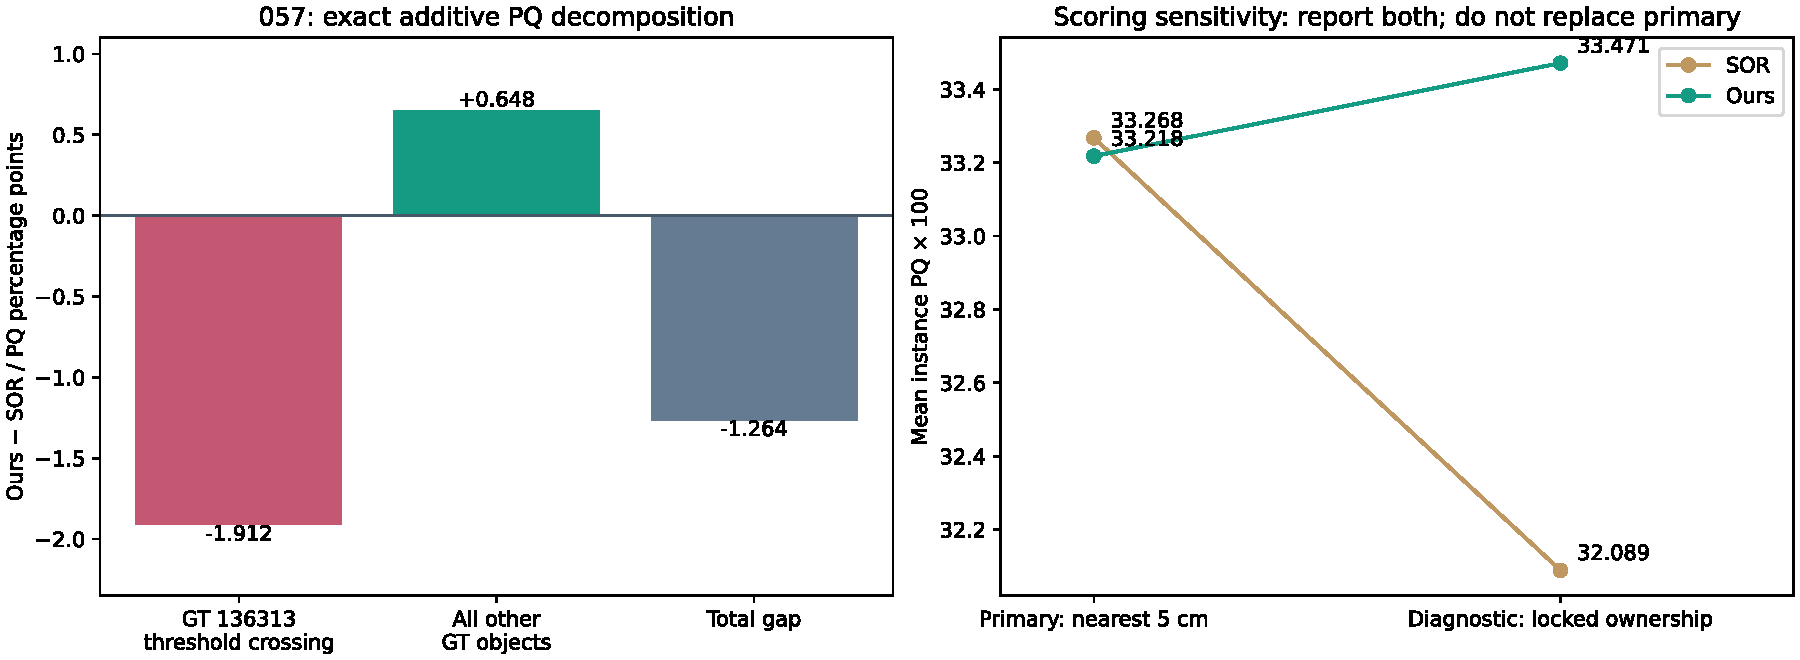
\includegraphics[width=.92\textwidth]{mechanism_decomposition.pdf}
\caption{The sequence-057 primary-score deficit relative to SOR decomposes into one SOR-only match and contributions from the remaining objects. The locked-assignment comparison changes the ranking, illustrating sensitivity to reference-label assignment; it does not replace the primary metric.}
\end{figure}

\begin{figure}[h!]
\centering
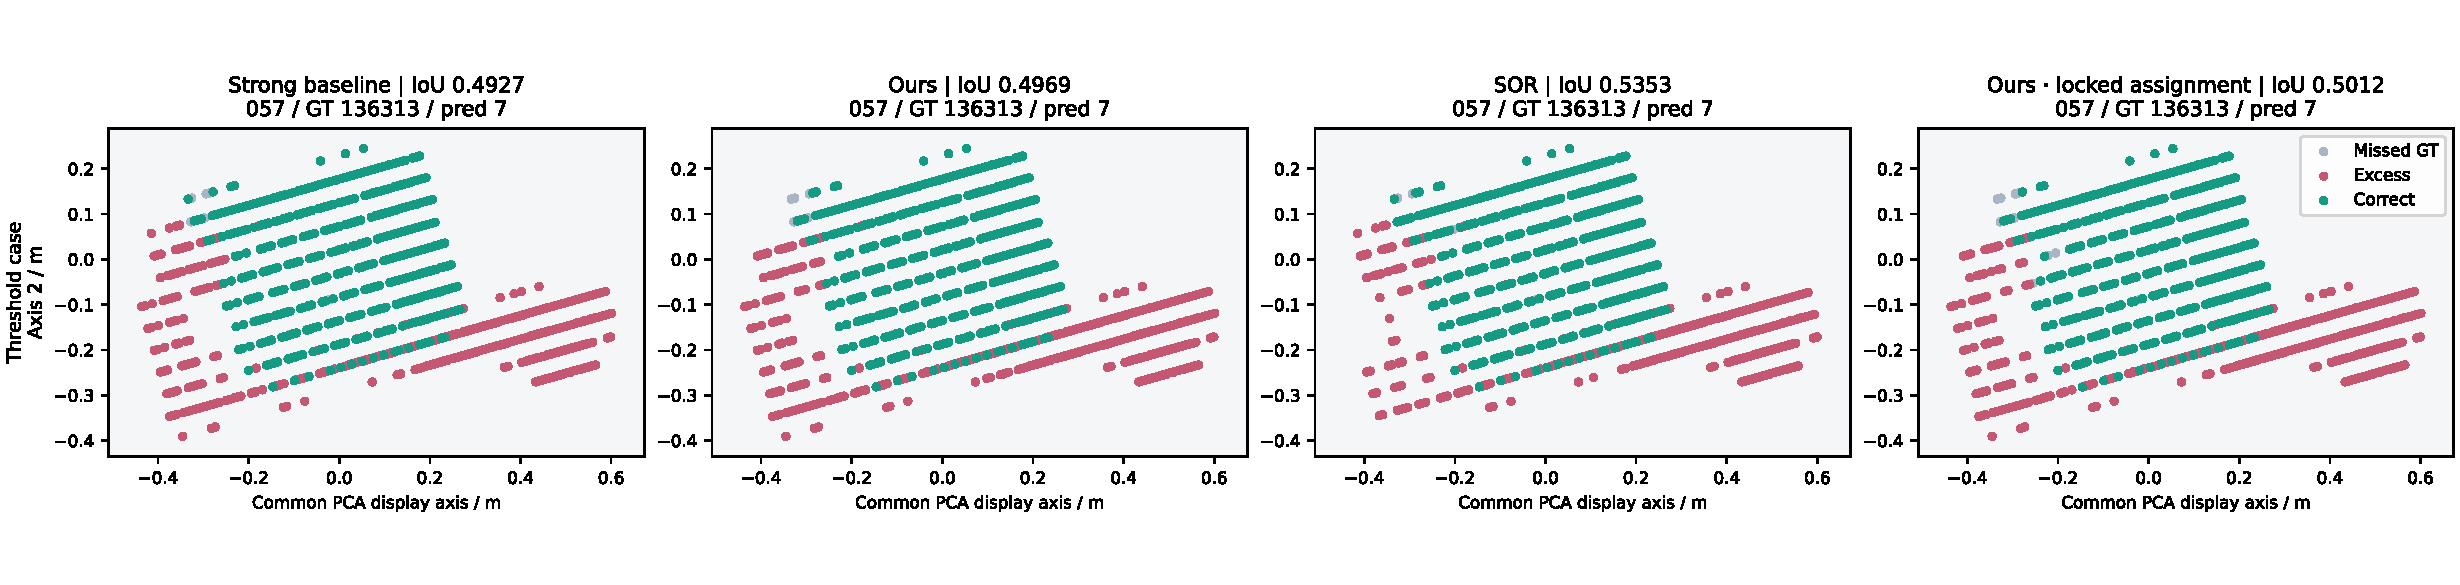
\includegraphics[width=.92\textwidth]{057_threshold_case.pdf}
\caption{Threshold-sensitive object in a shared projection. Correct, excess, and missed reference support use green, red, and gray, respectively. The fourth panel locks baseline nearest-source ownership before deletion.}
\end{figure}
